%Response
The federal reserve is responsible for constraining an out of control economic expansion.  The job of the federal reserve is to 'pull away the punch bowl, just when the party is getting good!'  The response of the federal reserve to the economic build up in years preceding the financial crisis of 2008, can be seen in the figures below.

\begin{figure}[H]
\centering
\begin{subfigure}{.5\textwidth}
  \centering
  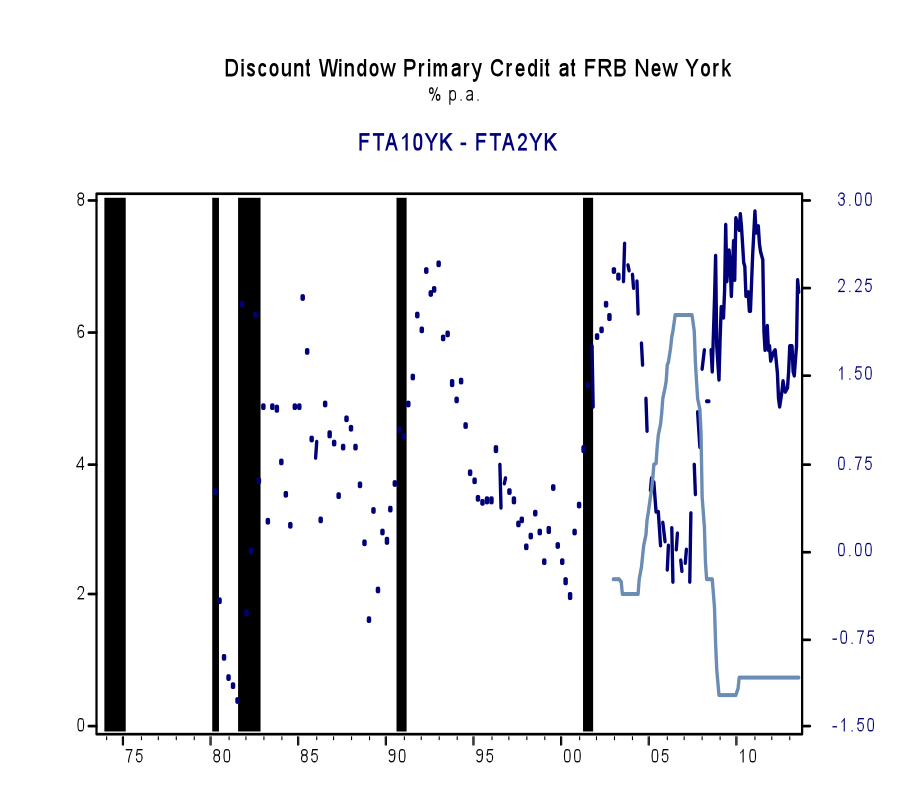
\includegraphics[width=1.0\linewidth]{figure/DiscountWindow.png}
  \caption{Discount Window Rate}%Firms Buying on Margin: On Behalf of Clients
  \label{fig:discountW}
\end{subfigure}%
\begin{subfigure}{.5\textwidth}
  \centering
  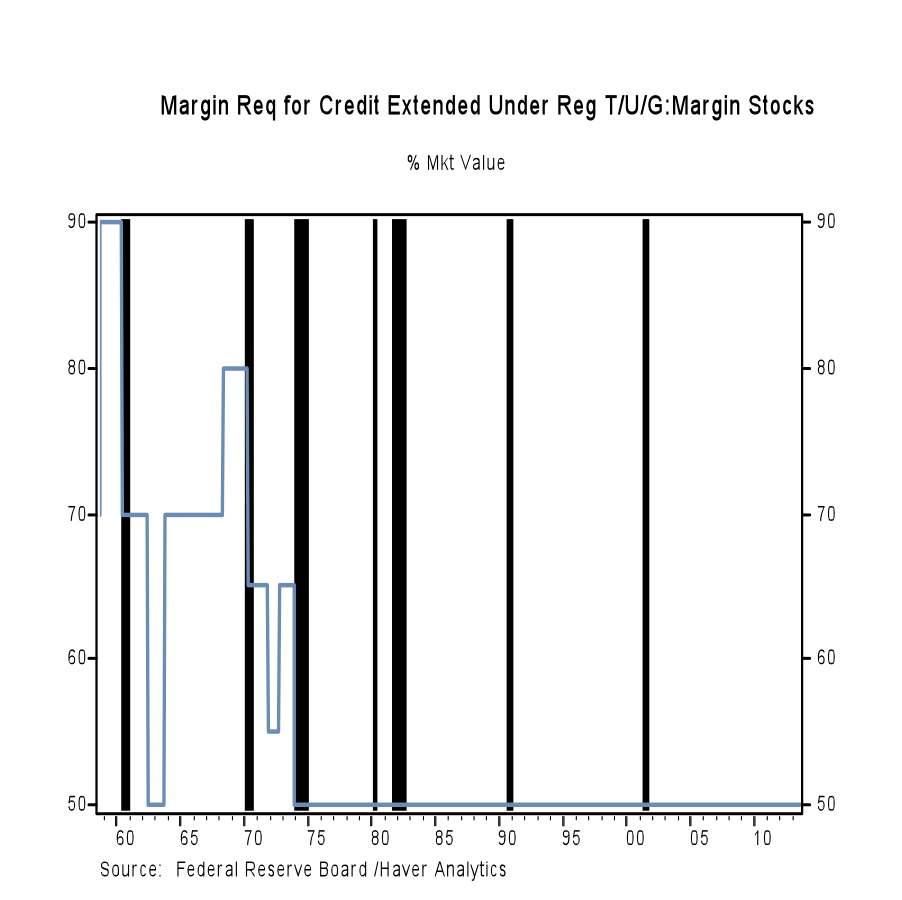
\includegraphics[width=1.0\linewidth]{figure/MarginStocks.png}
  \caption{Margin Requirement on Credit for Stocks}
  \label{fig:stocks}
\end{subfigure}
\caption{Responses in a Treasury Yield Inversion}
\label{fig:NEW2}
\end{figure}

There is major disagreement about criteria of policy, varying from emphasis on money market conditions, interest rates, and the quantity of money to the belief that the state of employment itself should be the proximate criterion of policy.\cite{Friedman} Following this line of thought, the execution of discount window primary credit rate hikes by the federal reserve were ill timed.  Actions by the federal reserve need to be more targeted in the highly leveraged and unstable economy that had been building prior to the financial crisis of 2008.

%%
%%Unemployment had again to be explained by rigidities or imperfections,not as the natural outcome of a fully operative market process. \cite{Friedman}
%%
%%Having detected such opportunities, those funds construct arbitrage trading strategies to profit: they buy securities that are underpriced and sell those that are overpriced, while simultaneously taking offsetting positions to hedge against any risks involved and lock in their arbitrage profits. \cite{Dowd}
%%
%%
%% ---market imperfections are there in TBTF to support individual Wealth of the nation's people, but the results of poor market discipline lead to worse off employment situations
%%
%%Milton Friedman revival to understand what monetary policy can do to protect the people.
%%Charts of noticeable Regulator Effects
%%Use some of the more refined tools in fractional banking to address the margin growth and maintain financial stability in asset valuation.  This is of pivotal importance in the growing bailout regime we have entered.  
%%
%%
%%
%%
%%
%%
%%
%%Build up Charts --- Showing that there was this behind the scenes effect that badly mixed with the inverted Yield Curve
%%Built up misnomer that the assets being held have increasing value....
%%
%%
